\begin{sloppypar*}

    The overall idea of the concept presented in this paper can be summarised in
    the \textit{mindmap} in Figure \ref{fig:mindmap} and the pictorial representation of
    the core logic can be seen in Figure \ref{fig:logic}. The authors have proposed
    two \textbf{triplet formats}:
    
    \begin{enumerate}
        \item \verb|(gene/disease, uni-relation, heterogeneous entity)|
        \item \verb|(gene/disease, multi-relation, gene/disease)|
    \end{enumerate}
    
    \noindent Here, a \textbf{heterogeneous entity} can be anyone of \textit{chemical,
    mutation, pathway and phenotype}. For the \textbf{uni-relation} types, there
    are $11$ alternatives:
    \begin{enumerate}
        \item disease-chemical edge \textit{obtained from CTD}
        \item gene-chemical edge \textit{obtained from CTD}
        \item disease-pathway edge \textit{obtained from CTD}
        \item gene-pathway edge \textit{obtained from CTD}
        \item gene-disease edge \textit{obtained from CTD}
        \item disease-mutation edge \textit{obtained from DisGeNET}
        \item gene-mutation edge \textit{obtained from DisGeNET}
        \item disease-phenotype edge \textit{obtained from HPO}
        \item gene-phenotype edge \textit{obtained from HPO}
        \item gene-gene edge \textit{obtained from BioGRID}
        \item disease-disease edge \textit{obtained from BioSNAP}
    \end{enumerate}
    
    \noindent Similarly, for \textbf{multi-relation} there are multiple options
    (\textit{apparently}), but, for the example described in the paper, they have
    selected (from \textbf{AGAC} database) \textit{mutation type} as the multi-
    relation, where, it has three variants, \textit{viz.}:
    
    \begin{enumerate}
        \item loss-of-function mutation
        \item gain-of-function mutation
        \item complex mutation
    \end{enumerate}

    \noindent Along with \textbf{AGAC}, $7$ data-sources are used, namely,
    \textbf{BioGRID}, \textbf{BioSNAP}, \textbf{CTD}, \textbf{DisGeNET},
    \textbf{Disease-Ontology}, \textbf{HPO} and \textbf{NCBI}. Also, a step called
    \textit{concept normalisation} is performed where for each node
    type, different concept IDs are used, such as, \textbf{Entrez ID for
    \textit{gene}}, \textbf{MESH ID for \textit{disease}}, \textbf{SNPID for
    \textit{mutation}}, \textbf{KEGG ID for \textit{pathway}} and \textbf{HPO ID
    for \textit{phenotype}}.

    \begin{mybox}
        This paper uses something equivalent of learnt tensor/matrix decomposition!
    \end{mybox}

    Further, the authors have noted that, ``\textit{...matrix is
    natural to store uni-relational triple information, while tensor serves well
    for multi-relational triple}''.Thus, the matrix $\mathcal{W} \in \mathbb{R}^{n \times h}$
    for \textit{uni-relations} (with rows as gene/disease and coloumn as entity)
    and the sparse tensor $\mathcal{X} \in \mathbb{R}^{n \times n \times K}$
    for \textit{multi-relations} is built from the $7$ data-sources for each of
    the \textbf{two} \textit{triplet} formats.

    \noindent where,

    $\mathcal{G}$: Number of unique genes,

    $\mathcal{D}$: Number of unique diseases,

    $K$: Number of types for the multi-relation. In the example used, it is $3$,

    $n = \mathcal{G} + \mathcal{D}$,

    $h = \mathcal{G} + \mathcal{D} + \mathcal{M}$,
    
    \noindent The values in $\mathcal{W}$ are binary, and those in $\mathcal{X}$
    are linkage weights.\hfill \newline

    The solution proposed in this paper, for generating learned embeddings, is via
    a joint decomposition of the matrix $\mathcal{W}$ and the sparse tensor $mathcal{X}$.
    The computational algorithm (\textbf{Algorithm} \ref{alg:jdhmt})
    captures the solution (\textit{the learnt joint-decomposition}):

    \begin{algorithm}
        \SetKwInOut{KwIn}{Input}
        \SetKwInOut{KwOut}{Output}
    
        \KwIn{The tensor $\mathcal{X}$ containing multi-relational triples, the 
        matrix $\mathcal{W}$ containing uni-relational triples.}
        \KwOut{$A$ (A coupled decomposed embedding matrix preserving both semantics
        from tensor $\mathcal{X}$ and $\mathcal{W}$), $V$, $C$).}
    
        \tcc{In the matrix $\mathcal{W}$, row indices are mapped to genes/diseases
        and coloumn indices are mapped to heterogeneous entities. The cell values
        are binary for uni-relation present/absent. In the sparse tensor
        $\mathcal{X}$, rows and coloumns denote genes/disease indices, and the
        third dimension is mapped to multi-relation type}

        %\tcp{} single line C style comment, on its own line
        %\tcp*[f]{} single line C style comment, at end of a code line
        
        Initialize $A$, $V$, $\mathcal{C}$.
        
        \Repeat{
            % End condition
            $\mathcal{J}(\theta)$ convergence
        }{
            % Loop text
            Parameter tuning
            
            \For{
                % For condition
                $i$ in iteration
            }{
                % Loop text
                $A \gets A \cdot \frac{
                    \lambda_{\mathcal{X}} \sum_{k=1}^{K} (\mathcal{X}_k A \mathcal{C}_k^T + \mathcal{X}_k^T A \mathcal{C}_k) + \lambda_W W V^T
                }{
                    \lambda_{\mathcal{X}} \sum_{k=1}^{K} (A \mathcal{C}_k^T A^T A \mathcal{C}_k + A \mathcal{C}_k A^T A \mathcal{C}_k^T) + \lambda_W A V V^T + \lambda_A A
                }$ \tcp*[f]{update rule for $A$}

                $V \gets V \cdot \frac{
                    \lambda_W A^T W
                }{
                    \lambda_W A^T A V + \lambda_V V
                }$  \tcp*[f]{update rule for $V$}

                $\mathcal{C}_k \gets \mathcal{C}_k \cdot \frac{
                    \sum_{k=1}^{K} A^T \mathcal{X}_k A
                }{
                    \sum_{k=1}^{K} (A^T A \mathcal{C}_k A^T A + \lambda_{\mathcal{C}} \mathcal{C}_k)
                }$ \tcp*[f]{update rule for $\mathcal{C}_k$}

                $i++$
            }
        } \tcp*[f]{here $\theta$ denotes the three parameters}

        \Return{$A$, $V$, $\mathcal{C}$}

        \caption{Computational algorithm for JDHMT model}\label{alg:jdhmt}
    \end{algorithm}

    \noindent In \textbf{Algorithm} \ref{alg:jdhmt}, the symbols have the following meaning,

    $\mathcal{J}(\theta) = f_{\mathcal{X}}(\mathcal{X}, A, \mathcal{C}) + f_{\mathcal{W}}(\mathcal{W}, A, V)$: 
    The objective function for \textit{convex optimization}

    $f_{\mathcal{X}}(\mathcal{X}, A, \mathcal{C}) = \lambda_{\mathcal{X}} \sum_{k=1}^{K} || \mathcal{X}_k - A \mathcal{C}_k A^T ||_{F}^{2} + \lambda_{\mathcal{C}} \sum_{k=1}^{K} || \mathcal{C}_k ||_{F}^{2}$:
    need to understand!

    $f_{\mathcal{W}}(\mathcal{W}, A, V) = \lambda_{\mathcal{W}} || \mathcal{W} - A V ||_{F}^{2} + \lambda_A || A ||_{F}^{2} + \lambda_V || V ||_{F}^{2}$:
    need to understand!
    
    $\theta = \{A, V, \mathcal{C}\}$: The parameter-set

    $A \in \mathbb{R}^{n \times e}$: need to understand!

    $V \in \mathbb{R}^{e \times h}$: need to understand!

    $\mathcal{C}_k = \mathcal{C}_{::k} \in \mathbb{R}^{e \times e}$: need to understand!

    \noindent All values in the matrix and the tensor are strictly non-negative.

    \begin{figure}
        \centering
        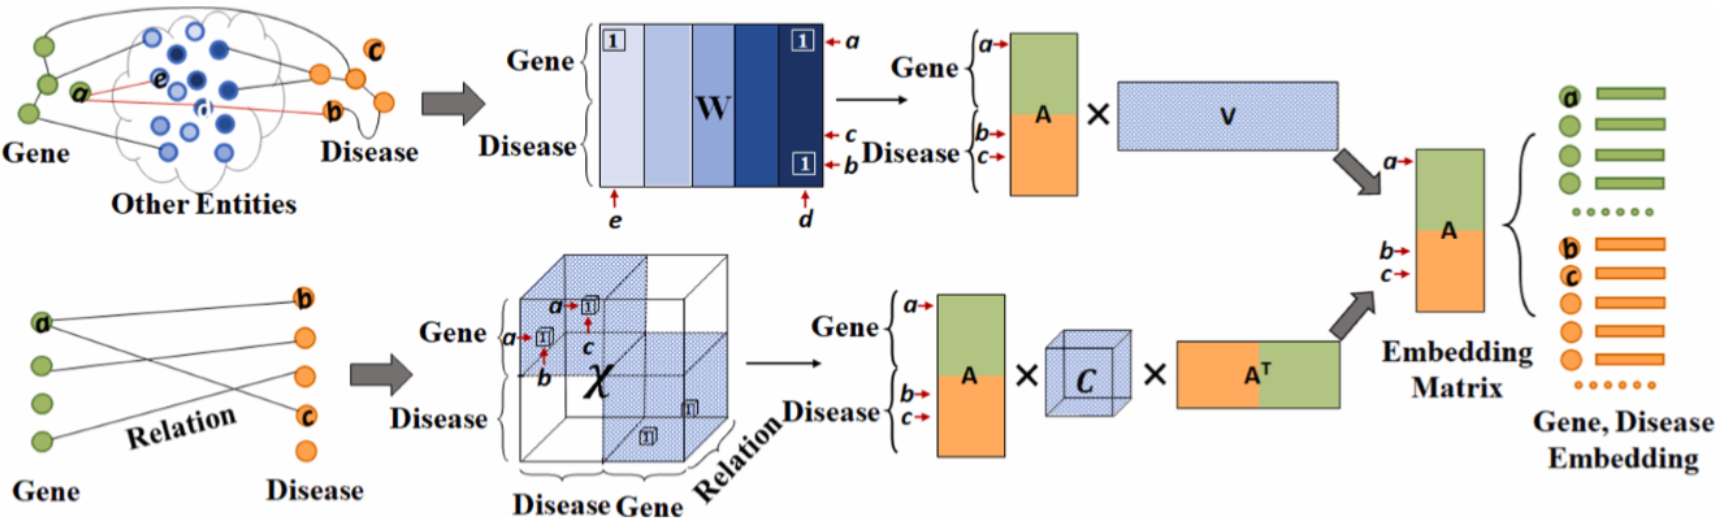
\includegraphics[width=170mm,scale=1]{jdhmt_core.png}
        \caption{The pictorial representation for Joint Decomposition of
        Heterogeneous Matrix and Tensor}
        \label{fig:logic}
    \end{figure}

    \begin{figure}
        \centering
        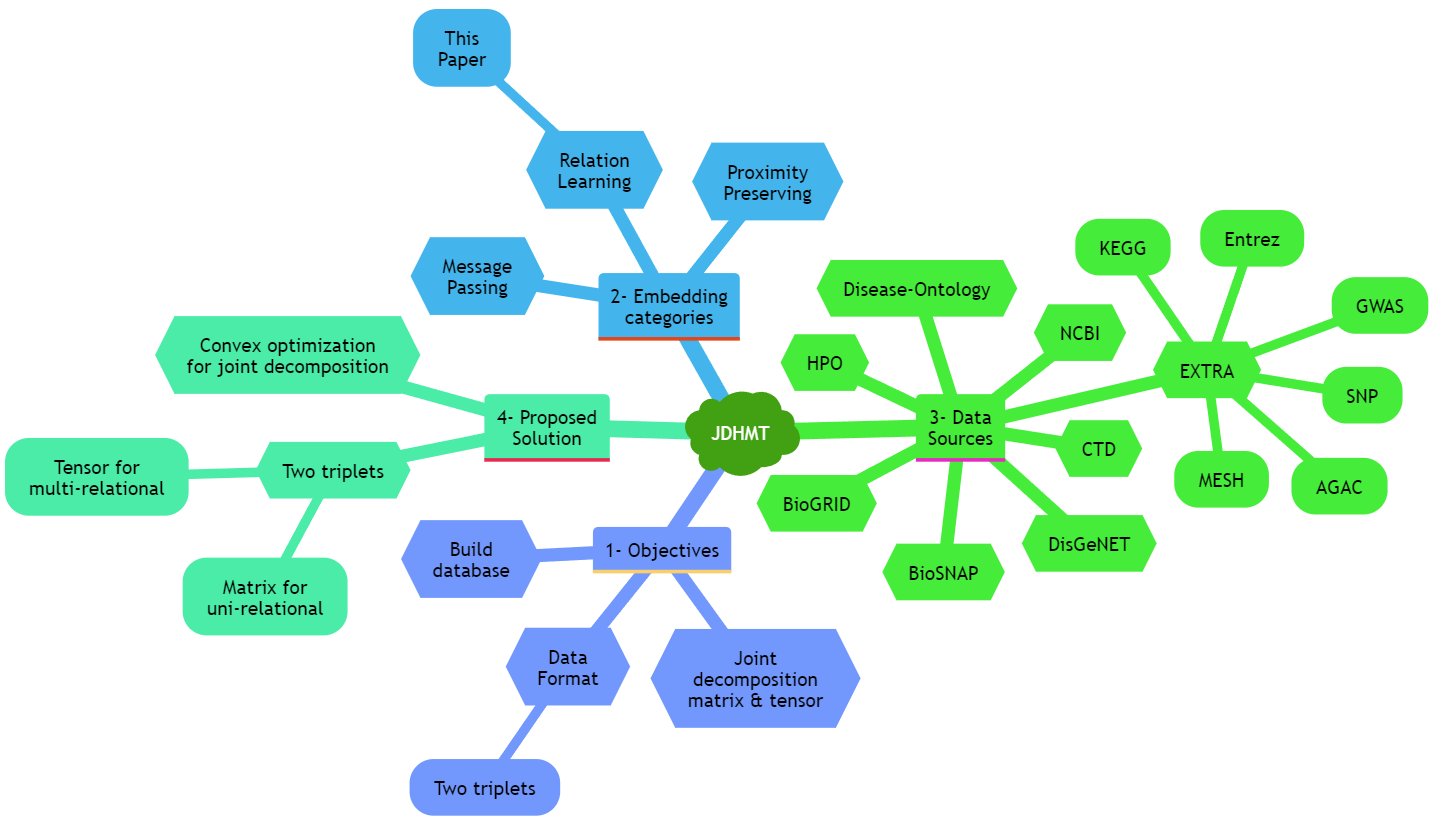
\includegraphics[width=170mm,scale=1]{mindmap.png}
        \caption{Mindmap}
        \label{fig:mindmap}
    \end{figure}
    
    % \begin{markdown}
    % \end{markdown}
    % \begin{figure}
    %     \centering
    %     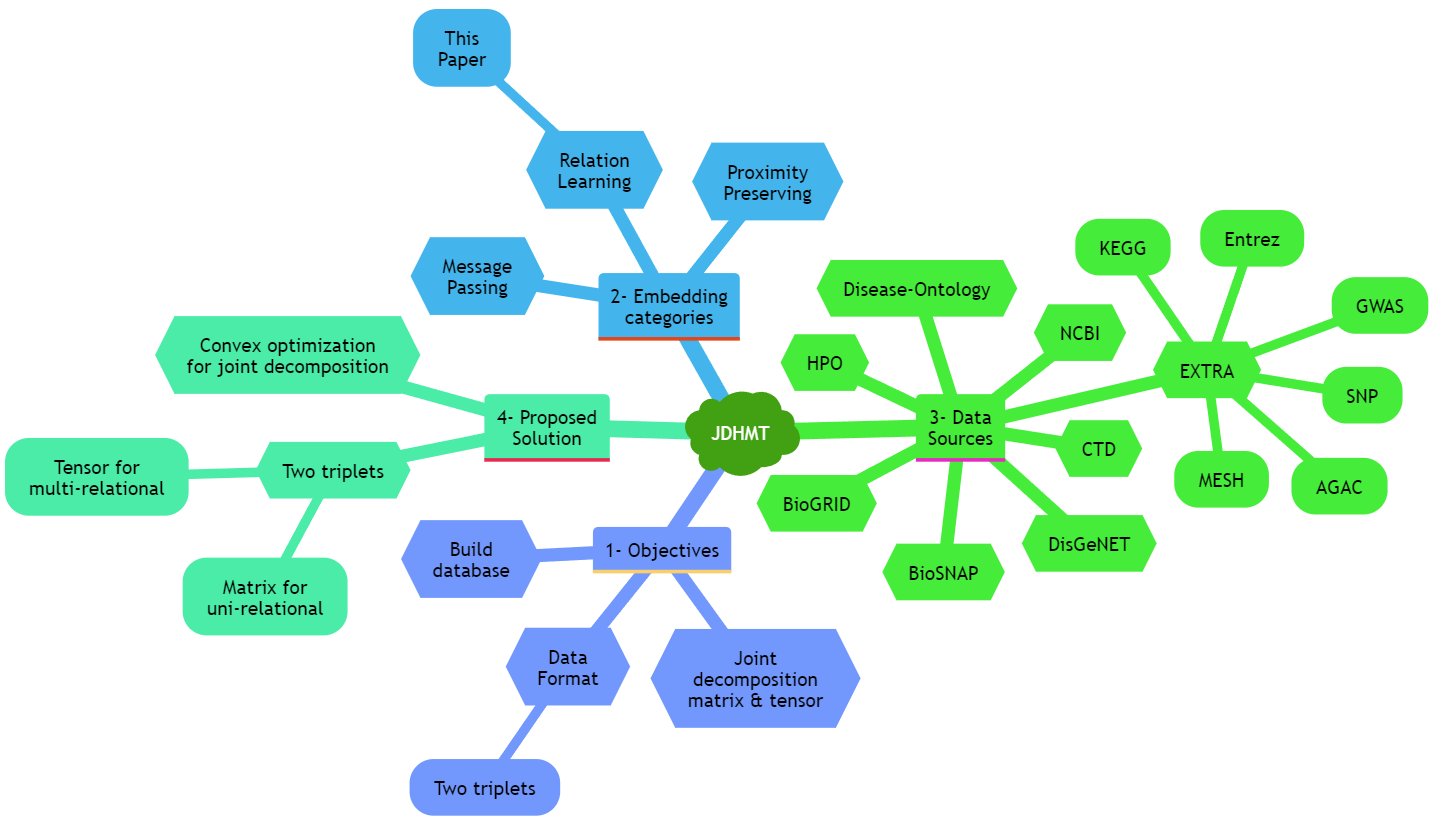
\includegraphics[width=170mm,scale=1]{mindmap.png}
    %     \caption{Mindmap}
    %     \label{fig:mindmap}
    % \end{figure}
    
    % For extrinsic evaluation, one of the tasks was link-prediction which is achieved
    % via tensor reconstruction from the decompositions.
    % \begin{equation*}
    %     \tilde{\mathcal{X}} = A \cdot \tilde{\mathcal{C}} \cdot A^{T}
    % \end{equation*}
    % \noindent In the above, the cell $\tilde{\mathcal{X}}_{ijk}$ denotes the
    % multi-relation triple ($gene_i$, $multi-relation_k$, $disease_j$).

    \begin{mybox}
        Since my study pertains to understanding the embedding generation, the
        intrinsic and extrinsic evaluations are not discussed.
    \end{mybox}
\end{sloppypar*}